\documentclass[12pt,french,oneside]{report}
%%%%%%%%%%%%%%%%%%%%%%%%%%%%%%%%%%%%%%%%%%%%%%%%%%%%%%%%%%%%%%%%%%%%%%%%%%%%%%%
\input{preambule_2015}
%___________________________
%===   Redéfinition des marges par défaut
%------------------------------------------------------
%\usepackage[textwidth=18.6cm]{geometry}%à mettre dans le preambule perso
%\pagestyle{fancy}%à mettre dans le preambule perso


\setlength\paperheight{297mm}
\setlength\paperwidth{210mm}
\setlength{\evensidemargin}{0cm}% Marge gauche sur pages paires
\setlength{\oddsidemargin}%{0cm}%
{-0.5cm}% Marge gauche sur pages impaires
\setlength{\topmargin}{-2cm}% Marge en haut
\setlength{\headsep}{0.5cm}% Entre le haut de page et le texte
\setlength{\headheight}{0.7cm}% Haut de page
\setlength{\textheight}{25.2cm}% Hauteur de la zone de texte
\setlength{\textwidth}{17cm}% Largeur de la zone de texte


% Environnement enumerate
\renewcommand{\theenumi}{\bf\textsf{\arabic{enumi}}}
\renewcommand{\labelenumi}{\bf\textsf{\theenumi.}}
\renewcommand{\theenumii}{\bf\textsf{\alph{enumii}}}
\renewcommand{\labelenumii}{\bf\textsf{\theenumii.}}
\renewcommand{\theenumiii}{\bf\textsf{\roman{enumiii}}}
\renewcommand{\labelenumiii}{\bf\textsf{\theenumiii.}}


\usetikzlibrary{shadows,trees}


%definition des couleurs
\definecolor{fondpaille}{cmyk}{0,0,0.1,0}%\pagecolor{fondpaille}
\definecolor{gris}{rgb}{0.7,0.7,0.7}
\definecolor{rouge}{rgb}{1,0,0}
\definecolor{bleu}{rgb}{0,0,1}
\definecolor{vert}{rgb}{0,1,0}
\definecolor{deficolor}{HTML}{2D9AFF}
\definecolor{backdeficolor}{HTML}{EDEDED}%{036DD0}%dégradé bleu{666666}%dégradé gris
\definecolor{theocolor}{HTML}{036DD0}%F4404D%rouge
\definecolor{backtheocolor}{HTML}{D3D3D3}
\definecolor{methcolor}{HTML}{008800}%12BB05}
\definecolor{backmethcolor}{HTML}{FFFACD}
\definecolor{backilluscolor}{HTML}{EDEDED}
\definecolor{sectioncolor}{HTML}{221E1E}%{B2B2B2}%vert : {HTML}{008800}%{HTML}{2D9AFF}
\definecolor{subsectioncolor}{HTML}{221E1E}%{B2B2B2}%vert : {HTML}{008800}%{rgb}{0.5,0,0}
\definecolor{engcolor}{HTML}{D4D7FE}
\definecolor{exocolor}{rgb}{0,0.6,0}
\definecolor{exosoltitlecolor}{rgb}{0,0.6,0}
\definecolor{titlecolor}{rgb}{1,1,1}

%commande pour enlever les couleurs avant impression
\newcommand{\nocolor}
{\pagecolor{white}
\definecolor{gris}{rgb}{0.7,0.7,0.7}
\definecolor{rouge}{rgb}{0,0,0}
\definecolor{bleu}{rgb}{0,0,0}
\definecolor{vert}{rgb}{0,0,0}
\definecolor{deficolor}{HTML}{B2B2B2}
\definecolor{backdeficolor}{HTML}{EEEEEE}%{036DD0}%dégradé bleu{666666}%dégradé gris
\definecolor{theocolor}{HTML}{B2B2B2}
\definecolor{backtheocolor}{HTML}{EEEEEE}
\definecolor{methcolor}{HTML}{B2B2B2}
\definecolor{backmethcolor}{HTML}{EEEEEE}
\definecolor{backilluscolor}{HTML}{EEEEEE}
\definecolor{sectioncolor}{HTML}{B2B2B2}
\definecolor{subsectioncolor}{HTML}{B2B2B2}
\definecolor{engcolor}{HTML}{EEEEEE}
\definecolor{exocolor}{HTML}{3B3838}
\definecolor{exosoltitlecolor}{rgb}{0,0,0}
\definecolor{titlecolor}{rgb}{0,0,0}
}



%___________________________
%===    Exercice résolu
%------------------------------------------------------
%
%#1 : énoncé
%#2 : solution
\newcounter{exosol}
\newcommand{\exosol}[2]{
\stepcounter{exosol}
\begin{tikzpicture}[node distance=0 cm]
\node[fill=backilluscolor,rounded corners=2pt,anchor=south west] (illus) at (0,-0.02)
{\it \textbf{\textcolor{exosoltitlecolor}{Exercice résolu \arabic{exosol}~:~}}};
\node[fill=backilluscolor,rounded corners=2pt,anchor=north west]at(0,0)
{\parbox{\columnwidth-10pt}{#1\par\medskip{\it \textbf{\textcolor{exosoltitlecolor}{Solution~:~}}}\par#2 }};
\end{tikzpicture}
\bigskip
}

\newcommand{\suite}[1]{
\begin{tikzpicture}[node distance=0 cm]
\node[fill=backilluscolor,rounded corners=2pt,anchor=north west]at(0,0)
{\parbox{\columnwidth-10pt}{{\it \textbf{\textcolor{exosoltitlecolor}{Suite de la solution~:}}}\par#1}};
\end{tikzpicture}
\bigskip
}



%%%%%%%%%%%%%%%%%%%%%%%%%%%%%%%%%%%%%%%%%%%%%%%%%%%%%%%%%%%%%%%%%%%%%%%%%%%%%%%
%Encadrés pour Propriétés, Théorème, Définitions, exemples, exercices

\usepackage{environ}%pour pouvoir utiliser la commande \NewEnviron

%___________________________
%===    Propriété avec ou sans s et avec ou sans titre
%------------------------------------------------------
%
\NewEnviron{Prop}[2][]{
\begin{tikzpicture}[node distance=0 cm]
\node[fill=theocolor,rounded corners=5pt,anchor=south west] (theorem) at (0,0)
{\textcolor{titlecolor}{Propriété#1~:~#2}};
\node[draw,drop shadow,color=theocolor,very thick,fill=backtheocolor,rounded corners=5pt,anchor=north west] at(0,-0.02)
{\black\parbox{\columnwidth-12pt}{\BODY}};
\end{tikzpicture}
\bigskip
}


%___________________________
%===    Conséquence avec ou sans s et avec ou sans titre
%------------------------------------------------------
%
\NewEnviron{Cons}[2][]{
\begin{tikzpicture}[node distance=0 cm]
\node[fill=theocolor,rounded corners=5pt,anchor=south west] (theorem) at (0,0)
{\textcolor{titlecolor}{Conséquence#1~:~#2}};
\node[draw,drop shadow,color=theocolor,very thick,fill=backtheocolor,rounded corners=5pt,anchor=north west] at(0,-0.02)
{\black\parbox{\columnwidth-12pt}{\BODY}};
\end{tikzpicture}
\bigskip
}


%___________________________
%===    Théorème avec ou sans titre
%------------------------------------------------------
%
\NewEnviron{Thm}[1][]{
\begin{tikzpicture}[node distance=0 cm]
\node[fill=theocolor,rounded corners=5pt,anchor=south west] (theorem) at (0,0)
{\textcolor{titlecolor}{Théorème~:~#1}};
\node[draw,drop shadow,color=theocolor,very thick,fill=backtheocolor,rounded corners=5pt,anchor=north west] at(0,-0.02)
{\black\parbox{\columnwidth-12pt}{\BODY}};
\end{tikzpicture}
\medskip
}


%___________________________
%===    Cadre arrondi coloré
%------------------------------------------------------
%
\NewEnviron{CadreColor}{

\begin{tikzpicture}[node distance=0 cm]
\node[draw,drop shadow,color=theocolor,very thick,fill=backtheocolor,rounded corners=5pt,anchor=north west] at(0,-0.02)
{\black\parbox{\columnwidth-12pt}{\BODY}};
\end{tikzpicture}
\medskip
}


%___________________________
%===    Cadre arrondi blanc
%------------------------------------------------------
%
\NewEnviron{Cadre}{
\begin{tikzpicture}[node distance=0 cm]
\node[draw,very thick,rounded corners=5pt,anchor=north west] at(0,-0.02)
{\black\parbox{\columnwidth-12pt}{\BODY}};
\end{tikzpicture}
\medskip
}



%___________________________
%===    Règle(s) avec ou sans s et avec sans titre
%------------------------------------------------------
%
\NewEnviron{Regle}[2][]{
\begin{tikzpicture}[node distance=0 cm]
\node[fill=theocolor,rounded corners=5pt,anchor=south west] (theorem) at (0,0)
{\textcolor{titlecolor}{Règle#1~:~#2}};
\node[draw,drop shadow,color=deficolor,very thick,fill=backdeficolor,rounded corners=5pt,anchor=north west] at(0,-0.02)
{\black\parbox{\columnwidth-12pt}{\BODY}};
\end{tikzpicture}
\medskip
}

%___________________________
%===    Définition avec ou sans s et avec sans titre
%------------------------------------------------------
%
\NewEnviron{Defi}[2][]{
\begin{tikzpicture}[node distance=0 cm]
\node[fill=theocolor,rounded corners=5pt,anchor=south west] (theorem) at (0,0)
{\textcolor{titlecolor}{Définition#1~:~#2}};
\node[draw,drop shadow,color=deficolor,very thick,fill=backdeficolor,rounded corners=5pt,anchor=north west] at(0,-0.02)
{\black\parbox{\columnwidth-12pt}{\BODY}};
\end{tikzpicture}
\medskip
}

%___________________________
%===    Méthode avec ou sans s et avec sans titre
%------------------------------------------------------
%
\NewEnviron{Methode}[2][]{
\begin{tikzpicture}[node distance=0 cm]
\node[fill=theocolor,rounded corners=5pt,anchor=south west] (theorem) at (0,0)
{\textcolor{titlecolor}{Méthode#1~:~#2}};
\node[draw,drop shadow,color=methcolor,very thick,fill=backmethcolor,rounded corners=5pt,anchor=north west] at(0,-0.02)
{\black\parbox{\columnwidth-12pt}{\BODY}};
\end{tikzpicture}
\medskip
}


%___________________________
%===    Redéfinition de la commande \chapter{•}
%------------------------------------------------------
%
\makeatletter

\renewcommand{\@makechapterhead}[1]{
\begin{tikzpicture}
\node[fill=theocolor,rectangle,rounded corners=5pt]{%
\begin{minipage}{\linewidth}
\begin{center}
\vspace*{9pt}
\textcolor{titlecolor}{\Large \textsc{\textbf{Chapitre \thechapter \ : \ #1}}}
\vspace*{9pt}
\end{center}
\end{minipage}
};\end{tikzpicture}
}

\makeatother


%___________________________
%===    Exemple avec ou sans s et avec ou sans titre
%------------------------------------------------------
%
\NewEnviron{Exemple}[2][]{
\begin{tikzpicture}[node distance=0 cm]
\node[draw,drop shadow,color=methcolor,very thick,fill=backmethcolor,rounded corners=5pt,anchor=north west] at(0,-0.02)
{\black\parbox{\columnwidth-12pt}{\textbf{Exemple#1~:~#2}\\
\BODY}};
\end{tikzpicture}
\medskip
}

%___________________________
%===    Remarque avec ou sans s
%------------------------------------------------------
%
\NewEnviron{Rmq}[1][]{
\textbf{\large{Remarque#1 :}}\par
\BODY
\medskip
}

%___________________________
%===    Remarques numérotées R1, R2, etc...
%------------------------------------------------------
%
\newcounter{rem}\newcommand{\rem}{\refstepcounter{rem}\textbf{R \therem \ :}\xspace}

%___________________________
%===    Exercices du contrôle numérotés
%------------------------------------------------------
%
\newcounter{exercice}
\NewEnviron{Exercice}[1][]{
\refstepcounter{exercice}\textbf{\large{Exercice \theexercice \ :}}\hfill \textbf{#1}\par
\BODY
\medskip
}

%___________________________
%===    Exercices non numérotés
%------------------------------------------------------
%
\NewEnviron{Exo}[1][]{
\textbf{\large{Exercice #1 \ :}}\par
\BODY
\medskip
}

%___________________________
%===    Démonstration
%------------------------------------------------------
\NewEnviron{Demo}{%
\textit{\textbf{Démonstration.}}\par
\BODY
\strut\hfill$\square$
\medskip
}

%___________________________
%===    Commandes perso
%------------------------------------------------------
%
%\Leftrightarrow
\newcommand{\Lr}{\Leftrightarrow}

%Ancienne commande chapitre
\newcommand{\chapitre}[1]{
\begin{tikzpicture}
\node[fill=theocolor,rectangle,rounded corners=5pt]{%
\begin{minipage}{\linewidth}
\begin{center}
\vspace*{9pt}
\textcolor{titlecolor}{\Large \textsc{\textbf{#1}}}
\vspace*{9pt}
\end{center}
\end{minipage}
};
\end{tikzpicture}
\bigskip
}

%Pour les fiches : commande de Cécile
\newcommand{\Fiche}[2]{%
\begin{tikzpicture}
	\node[draw, color=blue,fill=white,rectangle,rounded corners=5pt]{%
	\begin{minipage}{\linewidth}
		\begin{center}
			\vspace*{9pt}
			\textcolor{blue}{\Large \textsc{\textbf{Fiche~#1\ :\ #2}}}
			\vspace*{7pt}
		\end{center}
	\end{minipage}
	};
\end{tikzpicture}
}%

\pagecolor{white}%couleur du fond de page

\renewcommand{\Pointilles}{%
\makebox[\linewidth]{\dotfill}
}


%centrer du texte ou une formule avec moins d'espace autour
\newcommand{\centrer}[1]
{
\smallskip
\centerline{#1}
\smallskip
}


%QRcode généré par le package qrcode
\usepackage{qrcode}


%Pour pouvoir utiliser l'environnement verbatim
\usepackage{verbatim}

%Panneau danger (nécessite le package pstricks)
\def\danger{\begingroup
\psset{unit=1ex}%
\begin{pspicture}(0,0)(3,3)
 
\pspolygon[linearc=0.2,linewidth=0.12,linecolor=red](0,0)(1.5,2.6)(3,0)
 
\psellipse*(1.5,1.33)(0.14,0.75)\pscircle*(1.5,0.3){0.15}\end{pspicture}
%
\endgroup}%

%___________________________
%===    Nouvelles commandes pour documents venant de Sesamath
%------------------------------------------------------
%
\definecolor{CyanTikz40}{cmyk}{.4,0,0,0}
\definecolor{CyanTikz20}{cmyk}{.2,0,0,0}
\tikzstyle{general}=[line width=0.3mm, >=stealth, x=1cm, y=1cm,line cap=round, line join=round]
\tikzstyle{quadrillage}=[line width=0.3mm, color=CyanTikz40]
\tikzstyle{quadrillageNIV2}=[line width=0.3mm, color=CyanTikz20]
\tikzstyle{quadrillage55}=[line width=0.3mm, color=CyanTikz40, xstep=0.5, ystep=0.5]
\tikzstyle{cote}=[line width=0.3mm, <->]
\tikzstyle{epais}=[line width=0.5mm, line cap=butt]
\tikzstyle{tres epais}=[line width=0.8mm, line cap=butt]
\tikzstyle{axe}=[line width=0.3mm, ->, color=Noir, line cap=rect]
\newcommand{\quadrillageSeyes}[2]{\draw[line width=0.3mm, color=A1!10, ystep=0.2, xstep=0.8] #1 grid #2;
\draw[line width=0.3mm, color=A1!30, xstep=0.8, ystep=0.8] #1 grid #2; }
\newcommand{\axeX}[4][0]{\draw[axe] (#2,#1)--(#3,#1); \foreach \x in {#4} {\draw (\x,#1) node {\small $+$}; \draw (\x,#1) node[below] {\small $\x$};}}
\newcommand{\axeY}[4][0]{\draw[axe] (#1,#2)--(#1,#3); \foreach \y in {#4} {\draw (#1, \y) node {\small $+$}; \draw (#1, \y) node[left] {\small $\y$};}}
\newcommand{\axeOI}[3][0]{\draw[axe] (#2,#1)--(#3,#1);  \draw (1,#1) node {\small $+$}; \draw (1,#1) node[below] {\small $I$};}
\newcommand{\axeOJ}[3][0]{\draw[axe] (#1,#2)--(#1,#3); \draw (#1, 1) node {\small $+$}; \draw (#1, 1) node[left] {\small $J$};}
\newcommand{\axeXgraduation}[2][0]{\foreach \x in {#2} {\draw (\x,#1) node {\small $+$};}}
\newcommand{\axeYgraduation}[2][0]{\foreach \y in {#2} {\draw (#1, \y) node {\small $+$}; }}
\newcommand{\origine}{\draw (0,0) node[below left] {\small $0$};}
\newcommand{\origineO}{\draw (0,0) node[below left] {$O$};}
\newcommand{\point}[4]{\draw (#1,#2) node[#4] {$#3$};}
\newcommand{\pointGraphique}[4]{\draw (#1,#2) node[#4] {$#3$};
\draw (#1,#2) node {$+$};}
\newcommand{\pointFigure}[4]{\draw (#1,#2) node[#4] {$#3$};
\draw (#1,#2) node {$\times$};}
\newcommand{\pointC}[3]{\draw (#1) node[#3] {$#2$};}
\newcommand{\pointCGraphique}[3]{\draw (#1) node[#3] {$#2$};
\draw (#1) node {$+$};}
\newcommand{\pointCFigure}[3]{\draw (#1) node[#3] {$#2$};
\draw (#1) node {$\times$};}


\definecolor{B1prime}                {cmyk}{0.00, 1.00, 0.00, 0.50}
\definecolor{H1prime}                {cmyk}{0.50, 0.00, 1.00, 0.00}

\definecolor{FootFonctionColor}{cmyk}{0.50, 0.00, 0.00, 0.00}
\definecolor{FootGeometrieColor}{cmyk}{0.40, 0.40, 0.00, 0.00}
\definecolor{FootStatistiqueColor}{cmyk}{0.30, 0.48, 0.00, 0.10}
\definecolor{FootStatistiqueOLDColor}{cmyk}{0.48, 0.30, 0.10, 0.00}
\definecolor{FootStatistique*Color}{cmyk}{0.20, 0.00, 0.00, 0.00}
\definecolor{ActiviteFootColor}{cmyk}{0.50, 0.00, 0.25, 0.00}
\definecolor{CoursFootColor}{cmyk}{0.15, 0.00, 0.00, 0.03}
\definecolor{ExoBaseFootColor}{cmyk}{0.00, 0.25, 0.50, 0.00}
\definecolor{ExoApprFootColor}{cmyk}{0.00, 0.25, 0.50, 0.00}
%\colorlet{ConnFootColor}{F2}
\definecolor{TPFootColor}{cmyk}{0.00, 0.30, 0.00, 0.10}
\definecolor{RecreationFootColor}{cmyk}{0.20, 0.00, 0.50, 0.05}

\definecolor{Blanc}             {cmyk}{0.00, 0.00, 0.00, 0.00}
\definecolor{Gris1}             {cmyk}{0.00, 0.00, 0.00, 0.20}
\definecolor{Gris2}             {cmyk}{0.00, 0.00, 0.00, 0.40}
\definecolor{Gris3}             {cmyk}{0.00, 0.00, 0.00, 0.50}
\definecolor{Noir}              {cmyk}{0.00, 0.00, 0.00, 1.00}
\definecolor{A1}              {cmyk}{0.33, 1.00, 0.00, 0.40}
\definecolor{F1}              {cmyk}{0.00, 1.00, 1.00, 0.00}
\definecolor{C1}              {cmyk}{0.00, 1.00, 0.00, 0.50}
\definecolor{G1}              {cmyk}{0.00, 0.00, 0.00, 0.20}
\definecolor{D1}              {cmyk}{0.00, 0.22, 0.49, 0.69}%bitume
\definecolor{J1}              {cmyk}{0.00, 0.34, 1.00, 0.02}%orangé


%augmenter l'espace au-dessus ou en-dessous d'une fraction
\usepackage{fixltx2e}
\makeatletter
\newcommand*\Strut[1][1]{%
  \leavevmode
  \vrule \@height #1\ht\strutbox
         \@depth #1\dp\strutbox
         \@width\z@
}
\newcommand*\TopStrut[1][1]{%
  \leavevmode
  \vrule \@height #1\ht\strutbox
         \@depth \z@
         \@width \z@
}
\newcommand*\BotStrut[1][1]{%
  \leavevmode
  \vrule \@height \z@
         \@depth #1\dp\strutbox
         \@width \z@
}
\makeatother


% coordonnées vecteurs dans le plan
%\newcommand{\covec2}[2]{\begin{pmatrix}#1\\#2\end{pmatrix}}


% coordonnées dans l'espace
%\newcommand{\covec3}[3]{\begin{pmatrix}#1\\#2\\#3\end{pmatrix}}

% QCM



%%%%%%%%%%%%%%%%%%%%%%%%%%%%%%%%%%%%%%%%%%%%%%%%%%%%%%%%%%%%%%%%%%%%%%%%%%%%%%%
\input{section_dom_2015_2016}
%%%%%%%%%%%%%%%%%%%%%%%%%%%%%%%%%%%%%%%%%%%%%%%%%%%%%%%%%%%%%%%%%%%%%%%%%%%%%%%

%entête classique

\fancypagestyle{garde_tete}{% 
%\fancyhead[C]{\small\textbf{\seconde} \hfill \small \textbf{Année 2015-2016}}
\renewcommand{\headrulewidth}{0cm}}

\newcommand{\tete}{
\thispagestyle{garde_tete}
\chapitre{Essais \LaTeX : figures avec Pstricks}

\noindent 
\vspace{-24pt}
}

%%%%%%%%%%%%%%%%%%%%%%%%%%%%%%%%%%%%%%%%%%%%%%%%%%%%%%%%%%%%%%%%%%%%%%%%%%%%%%%

%%%%%%%%%%%%%%%%%%%%%%%%%%%%%%%%%%%%%%%%%%%%%%%%%%%%%%%%%%%%%%%%%%%%%%%%%%%%%%%

%%%%%%%%%%%%%%%%%%%%%%%
%% DEBUT DU DOCUMENT %%
%%%%%%%%%%%%%%%%%%%%%%%

\begin{document}
\selectlanguage{french}
\setlength\parindent{0mm}
\tete 		%entête classique

\renewcommand \footrulewidth{0.2pt}%
\renewcommand \headrulewidth{0pt}%
\pagestyle{fancy}
\fancyhf{}
\pieddepage{\LaTeX}{}{\thepage / \pageref{LastPage}}

%%%%%%%%%%%%%%%%%%%%%%%%%%%%%%%%%%%%%%%%%%%%%%%%%%%%%%%%%%%%
\begin{spacing}{1.2}
%%%%%%%%%%%%%%%%%%%%%%%%%%%%%%%%%%%%%%%%%%%%%%%%%%%%%%%%%%%%

\section{Quadrillage petits carreaux}

\medskip

La macro suivante (ne nécessitant pas pstricks !) dessine un quadrillage à petits carreaux de longueur (modifiable) 17 cm (34 petits carreaux).

\def\quadri#1{\smallbreak\textcolor{gray}{\setlength\unitlength{5mm}\begin{picture}(36,#1)
\multiput(0,0)(1,0){37}{\line(0,1){#1}}
\put(0,0){\line(1,0){36}}
\multiput(0,1)(0,1){#1}{\line(1,0){36}}
\end{picture}}\medbreak}

Exemple d'utilisation : \verb~\quadribis{10}~

\quadri{10}

%**********************************************

La macro suivante dessine un quadrillage à petits carreaux de dimensions horizontalement \# 1 et verticalement \# 2. 

Exemple d'utilisation : \verb~\quadribis{8}{4}~

\newcommand\quadribis[2]{%\begin{center}
\setlength\unitlength{5mm}
\begin{minipage}{#1\unitlength}\smallbreak\textcolor{gray}{\begin{picture}(#1,#2)
\line(0,1){#2}
\multiput(1,0)(1,0){#1}{\line(0,1){#2}}
\put(0,0){\line(1,0){#1}}
\multiput(0,1)(0,1){#2}{\line(1,0){#1}}
\end{picture}}%\medbreak
\end{minipage}
%\end{center}
}

\quadribis{8}{4}



\section{Têtes d'animaux}

\medskip

%Serpent%%%%%%%%%%%%%%%%%%%%%%%%%%%%%%%%%%%%
\psset{unit=0.4cm}
\begin{pspicture}(0,0)(12,12)
\multido{\n=0+1}{13}{\psline(\n,0)(\n,12)}
\multido{\n=0+1}{13}{\psline(0,\n)(12,\n)}
{\psset{linewidth=2pt}
\pspolygon(0,2)(1,0)(10,0)(12,1)(12,3)(10,4)(7,3)(5,4)(6,7)(9,8)(10,8)(11,9)(7,10)(4,7)(4,3)(7,2)(10,3)(11,2)(10,1)(2,0.25)
\psline(6.75,7.75)(7,8)(9,8)
\pspolygon*(9,9)(8,9)(8,9.375)}
\end{pspicture}$\ $ \\

%Chien1%%%%%%%%%%%%%%%%%%%%%%%%%%%%%%%%%%%%
\psset{unit=0.4cm}
\begin{pspicture}(0,0)(12,12)
\multido{\n=0+1}{13}{\psline(\n,0)(\n,12)}
\multido{\n=0+1}{13}{\psline(0,\n)(12,\n)}
{\psset{linewidth=2pt}
\pspolygon(4,2)(6,2)(6,3)(7,4)(8,4)(9,5)(10,5)(11,6)(11,7)(9,7)(9,9)(8,10)(5,10)(3,8)(3,3)
\pspolygon*(3,4)(4,3)(5,3)(6,4)(5,5)(4,5)(3,6)
\pspolygon*(7,7)(8,7)(8,8)
\pspolygon*(10,7)(11,7)(11,6)
\psline(5,5)(5,8)
\psline(6,6)(8,6)
\psline(7,6)(8,5)(9,5)
\psline(8,8)(8,9)(7,9)(6,8)}
\end{pspicture}$\ $ \\

%Souris%%%%%%%%%%%%%%%%%%%%%%%%%%%%%%%%%%%%
\psset{unit=0.4cm}
\begin{pspicture}(0,0)(12,12)
\multido{\n=0+1}{13}{\psline(\n,0)(\n,12)}
\multido{\n=0+1}{13}{\psline(0,\n)(12,\n)}
{\psset{linewidth=2pt}
\psline(4,2)(4,5)
\psline(5,5)(1,5)(0,6)(0,8)(1,9)(3,9)
\pspolygon*(3,9)(5,7)(5,8)(6,7)(6,8)(9,8)(8,9)(6,9)(7,10)(6,10)(5,9)(5,10)(4,9)(4,10)
\pspolygon*(3,8)(2,8)(1,7)(2,6)(3,6)(2,7)(3,7)(4,6)(5,6)
\pspolygon*(2,5)(2,4)(3,5)
\pspolygon*(3,5)(3,3)(4,4)(4,5)
\psline(5,2)(7,4)
\psline(6,5)(7,4)(11,4)(11,3)(10,3)(10,4)(11,4)(12,5)(11,6)(10,6)(8,8)
\pspolygon*(12,5)(12,6)(11,6)
\pspolygon*(9,6)(8,6)(8,7)
\psline(8,7)(7,7)(7,6)(8,6)
\psline(7,5)(9,5)
\psline(8,5)(9,4)}
\pscircle*(10,5){0.15} \pscircle*(11,5){0.15}
\end{pspicture}$\ $ \\

%Poussin%%%%%%%%%%%%%%%%%%%%%%%%%%
\psset{unit=0.4cm}
\begin{pspicture}(0,0)(12,12)
\multido{\n=0+1}{13}{\psline(\n,0)(\n,12)}
\multido{\n=0+1}{13}{\psline(0,\n)(12,\n)}
{\psset{linewidth=2pt}
\psline(3,1)(1,1)(4,4)(5,4)(8,7)(10,7)(12,8)(10,10)(9,10)(6,7)(3,7)(2,9)(1,6)(1,5)(2,4)(2,2)
\psline(3,6)(2,5)(4,5)(5,6)
\psline(10,8)(12,8)
\psline(10,7)(10,8)(11,9)}
\pscircle*(10,9){0.25}
\end{pspicture}$\ $ \\

%Chat%%%%%%%%%%%%%%%%%%%%%%%%%%
\psset{unit=0.4cm}
\begin{pspicture}(0,0)(12,12)
\multido{\n=0+1}{13}{\psline(\n,0)(\n,12)}
\multido{\n=0+1}{13}{\psline(0,\n)(12,\n)}
{\psset{linewidth=2pt}
\psline(5,0)(5,2)(2,5)(2,7)(3,8)(3,10)(2,11)(2,12)(4,10)(8,10)(10,12)(10,11)(9,10)(9,8)(10,7)(10,5)(7,2)(7,0)
\psline(3,6)(3,5)(5,3)(5,4)(6,5)(7,4)(7,3)(9,5)(9,6)(8,7)
\psline(1,6)(4,6)
\psline(8,6)(12,6)
\psline(0,5)(4,5)
\psline(8,5)(11,5)
\psline(3,5)(4,5)
\psline(7,4)(8,4)
\psline(4,4)(5,4)
\psline(5,8)(6,9)
\psline(7,9)(8,8)}
\pspolygon*(6,5)(7,6)(5,6)
\pspolygon*(5,7)(5,8)(4,7)
\pspolygon*(7,8)(7,7)(8,8)
\pspolygon*(3,8)(2,9)(2,10)(3,9)
\pspolygon*(3,9.2)(2,10.2)(2,11)(3,10)
\pspolygon*(10,9)(9,8)(9,9)(10,10)
\pspolygon*(9,9.2)(9,10)(10,11)(10,10.2)
\pscircle*(5,5){0.2} \pscircle*(7,5){0.2}
\end{pspicture}$\ $ \\

%Chien2%%%%%%%%%%%%%%%%%%%%%%%%%%
\psset{unit=0.4cm}
\begin{pspicture}(0,0)(12,12)
\multido{\n=0+1}{13}{\psline(\n,0)(\n,12)}
\multido{\n=0+1}{13}{\psline(0,\n)(12,\n)}
{\psset{linewidth=2pt}
\pspolygon*(2,0)(3,0)(4,1)(4,2)(3,3)(2,3)(1,4)(1,1)
\pspolygon*(1,5)(1,8)(2,9)(2,6)
\pspolygon*(8,0)(9,0)(10,1)(10,8)(7,11)(6,11)(9,8)(9,2)(8,2)(8,5)(7,6)(7,1)
\pspolygon*(6,1)(6,2)(5,2)
\pspolygon*(3,5)(2,6)(4,6)
\pspolygon*(4,6)(4,7)(3,7)
\pspolygon*(6,6)(6,7)(5,7)
\pspolygon*(7,8)(8,7)(8,8)(7,9)
\psline(2,3)(3,4)(4,3)
\psline(2,3)(5,3)(6,4)(7,5)(7,6)
\psline(3,4)(3,5)
\psline(5,0)(5,1)(4,2)
\psline(4,6)(6,6)
\psline(3,6)(3,8)(4,8)
\psline(5,6)(5,8)(6,8)
\psline(1,4)(1,5)
\psline(7,6)(7,8)
\psline(2,9)(4,11)(6,11)}
\pscircle*(2,4){0.15} \pscircle*(4,4){0.15} \pscircle*(5,4){0.15}
\pscircle*(2,5){0.15} \pscircle*(4,5){0.15} \pscircle*(5,5){0.15}
\end{pspicture}$\ $ \\

%Renard%%%%%%%%%%%%%%%%%%%%%%%%%%
\psset{unit=0.4cm}
\begin{pspicture}(0,0)(12,12)
\multido{\n=0+1}{13}{\psline(\n,0)(\n,12)}
\multido{\n=0+1}{13}{\psline(0,\n)(12,\n)}
{\psset{linewidth=2pt}
\psline(0,2)(1,3)(1,2)(2,1)(2,3)(3,2)(3,3)(4,3)(5,4)(7,4)(8,5)(8,4)(9,5)(9,4)(12,7)(7,7)(4,10)(5,11)(7,11)(6,12)(2,12)(0,10)(0,9)
\psline(1,7)(2,8)(2,9)(5,12)
\psline(0,5)(0,3)(1,4)(1,3)
\psline(3,3)(3,4)
\psline(3,6)(5,6)
\psline(4,6)(4,5)(5,4)
\psline(8,5)(10,5)
\psline(3,8)(4,9)(5,8)(4,8)(4,7)(5,7)
\pspolygon*(5,7)(6,7)(5,8)
\pspolygon*(3,10)(4,10)(5,11)(7,11)(6,12)(5,12)
\pspolygon*(10,7)(10,6)(11,6)(12,7)}
\pscircle*(3,5){0.15} \pscircle*(5,5){0.15} \pscircle*(6,5){0.15} \pscircle*(6,6){0.15} \pscircle*(7,5){0.15} \pscircle*(7,6){0.15} \pscircle*(8,6){0.15}
\end{pspicture}$\ $ \\



\section{Rapporteurs}

\medskip

\psset{unit=1.5cm}
\pspicture(-2.5,-0.75)(2.5,2.5)
\SpecialCoor
\psarc(0,0){2.5}{0}{180}
\psline(-2.5,0)(-2.5,-0.75)(2.5,-0.75)(2.5,0)
\psarc(0,0){1.5}{0}{180}
\psline(0.25,0)(1.5,0)
\psarc(0,0){0.25}{0}{180}
\psline(-1.5,0)(-0.25,0)
\psline(-0.1,0)(0.1,0) \psline(0,-0.1)(0,0.1)
\multido{\i=0+2}{90}{\psline(2.25;\i)(2.5;\i)}
\multido{\i=0+10}{19}{\psline(2.125;\i)(2.5;\i)}
\multido{\i=0+20}{10}{\uput[\i](1.725;\i){\footnotesize{\i}}}
\multido{\i=10+20}{9}{\uput[\i](1.725;\i){\footnotesize{\i}}}
\endpspicture

\medskip

************************

\medskip

\psset{unit=2.5cm}
\pspicture(-3.125,-0.5)(3.125,2.875)
\SpecialCoor
\psarc(0,0){2.5}{0}{180}
\psline(-2.5,0)(-2.5,-0.5)(2.5,-0.5)(2.5,0)
\psarc(0,0){1.375}{0}{180}
\psline(0.25,0)(1.375,0)
\psarc(0,0){0.25}{0}{180}
\psline(-1.375,0)(-0.25,0)
\psline(-0.1,0)(0.1,0) \psline(0,-0.1)(0,0.1)
\multido{\i=0+10}{19}{\psline(2.25;\i)(2.5;\i)}
\multido{\i=0+20}{10}{\uput[\i](1.925;\i){\normalsize{\i}}}
\multido{\i=10+20}{9}{\uput[\i](1.925;\i){\normalsize{\i}}}
\multido{\i=180+-10,\I=0+10}{10}{\uput[\i](1.6;\i){\normalsize{\I}}}
\multido{\i=90+-10,\I=90+10}{10}{\uput[\i](1.6;\i){\normalsize{\I}}}
\multido{\i=0+2}{90}{\psline(1.375;\i)(1.5;\i)}
\multido{\i=0+10}{19}{\psline(1.375;\i)(1.625;\i)}
\multido{\i=0+1}{180}{\psline[linewidth=0.8pt](2.375;\i)(2.5;\i)}
\multido{\i=0+5}{36}{\psline(2.335;\i)(2.5;\i)}
\multido{\i=0+2}{90}{\psline[linewidth=0.2pt](1.375;\i)(1.5;\i)}
\multido{\i=1+2}{90}{\psline[linewidth=0.1pt](1.375;\i)(1.45;\i)}
\endpspicture

\medskip

************************

\medskip

\newcommand{\DemiTour}[1]{\rotatebox[origin=c]{180}{#1}}
\psset{unit=1.675cm}
\pspicture(-2.5,-2.5)(2.5,2.5)
\SpecialCoor
\pscircle(0,0){2.5}
\pscircle(0,0){1.5}
\psline(0.25,0)(1.75,0)
\pscircle(0,0){0.25}
\psline(-1.75,0)(-0.25,0)
\psline(-0.1,0)(0.1,0) \psline(0,-0.1)(0,0.1)
\multido{\i=0+2}{180}{\psline(2.25;\i)(2.5;\i)}
\multido{\i=0+10}{37}{\psline(2.125;\i)(2.5;\i)}
\multido{\i=0+10}{19}{\psline(2.125;\i)(2.5;\i)}
\multido{\i=0+20}{10}{\uput[\i](1.725;\i){\footnotesize{\i}}}
\multido{\i=10+20}{9}{\uput[\i](1.725;\i){\footnotesize{\i}}}
\uput[350](1.725;350){\footnotesize{\DemiTour{10}}}
\uput[340](1.725;340){\footnotesize{\DemiTour{20}}}
\uput[330](1.725;330){\footnotesize{\DemiTour{30}}}
\uput[320](1.725;320){\footnotesize{\DemiTour{40}}}
\uput[310](1.725;310){\footnotesize{\DemiTour{50}}}
\uput[300](1.725;300){\footnotesize{\DemiTour{60}}}
\uput[290](1.725;290){\footnotesize{\DemiTour{70}}}
\uput[280](1.725;280){\footnotesize{\DemiTour{80}}}
\uput[270](1.725;270){\footnotesize{\DemiTour{90}}}
\uput[260](1.725;260){\footnotesize{\DemiTour{100}}}
\uput[250](1.725;250){\footnotesize{\DemiTour{110}}}
\uput[240](1.725;240){\footnotesize{\DemiTour{120}}}
\uput[230](1.725;230){\footnotesize{\DemiTour{130}}}
\uput[220](1.725;220){\footnotesize{\DemiTour{140}}}
\uput[210](1.725;210){\footnotesize{\DemiTour{150}}}
\uput[200](1.725;200){\footnotesize{\DemiTour{160}}}
\uput[190](1.725;190){\footnotesize{\DemiTour{170}}}
\endpspicture


\section{Touches de calculatrice}

\medskip

\newcommand\tc[1]{%
{\psset{unit=0.35cm}
\begin{pspicture}(-1,-1)(1,1)
\psframe[framearc=0.5](-1,-1)(1,1)
\rput(0,0){$\mathtt{#1}$}
\end{pspicture}}}

\tc{1}

\tc{trigonométrie}



%%%%%%%%%%%%%%%%%%%%%%%%%%%%%%%%%%%%%%%%%%%%%%%%%%%%%%%%%%%%
\end{spacing}
%%%%%%%%%%%%%%%%%%%%%%%%%%%%%%%%%%%%%%%%%%%%%%%%%%%%%%%%%%%%
%%%%%%%%%%%%%%%%%%%%%
%% FIN DU DOCUMENT %%
%%%%%%%%%%%%%%%%%%%%%
\end{document}